\section{Introduction}

\begin{figure}[t]
    \centering
    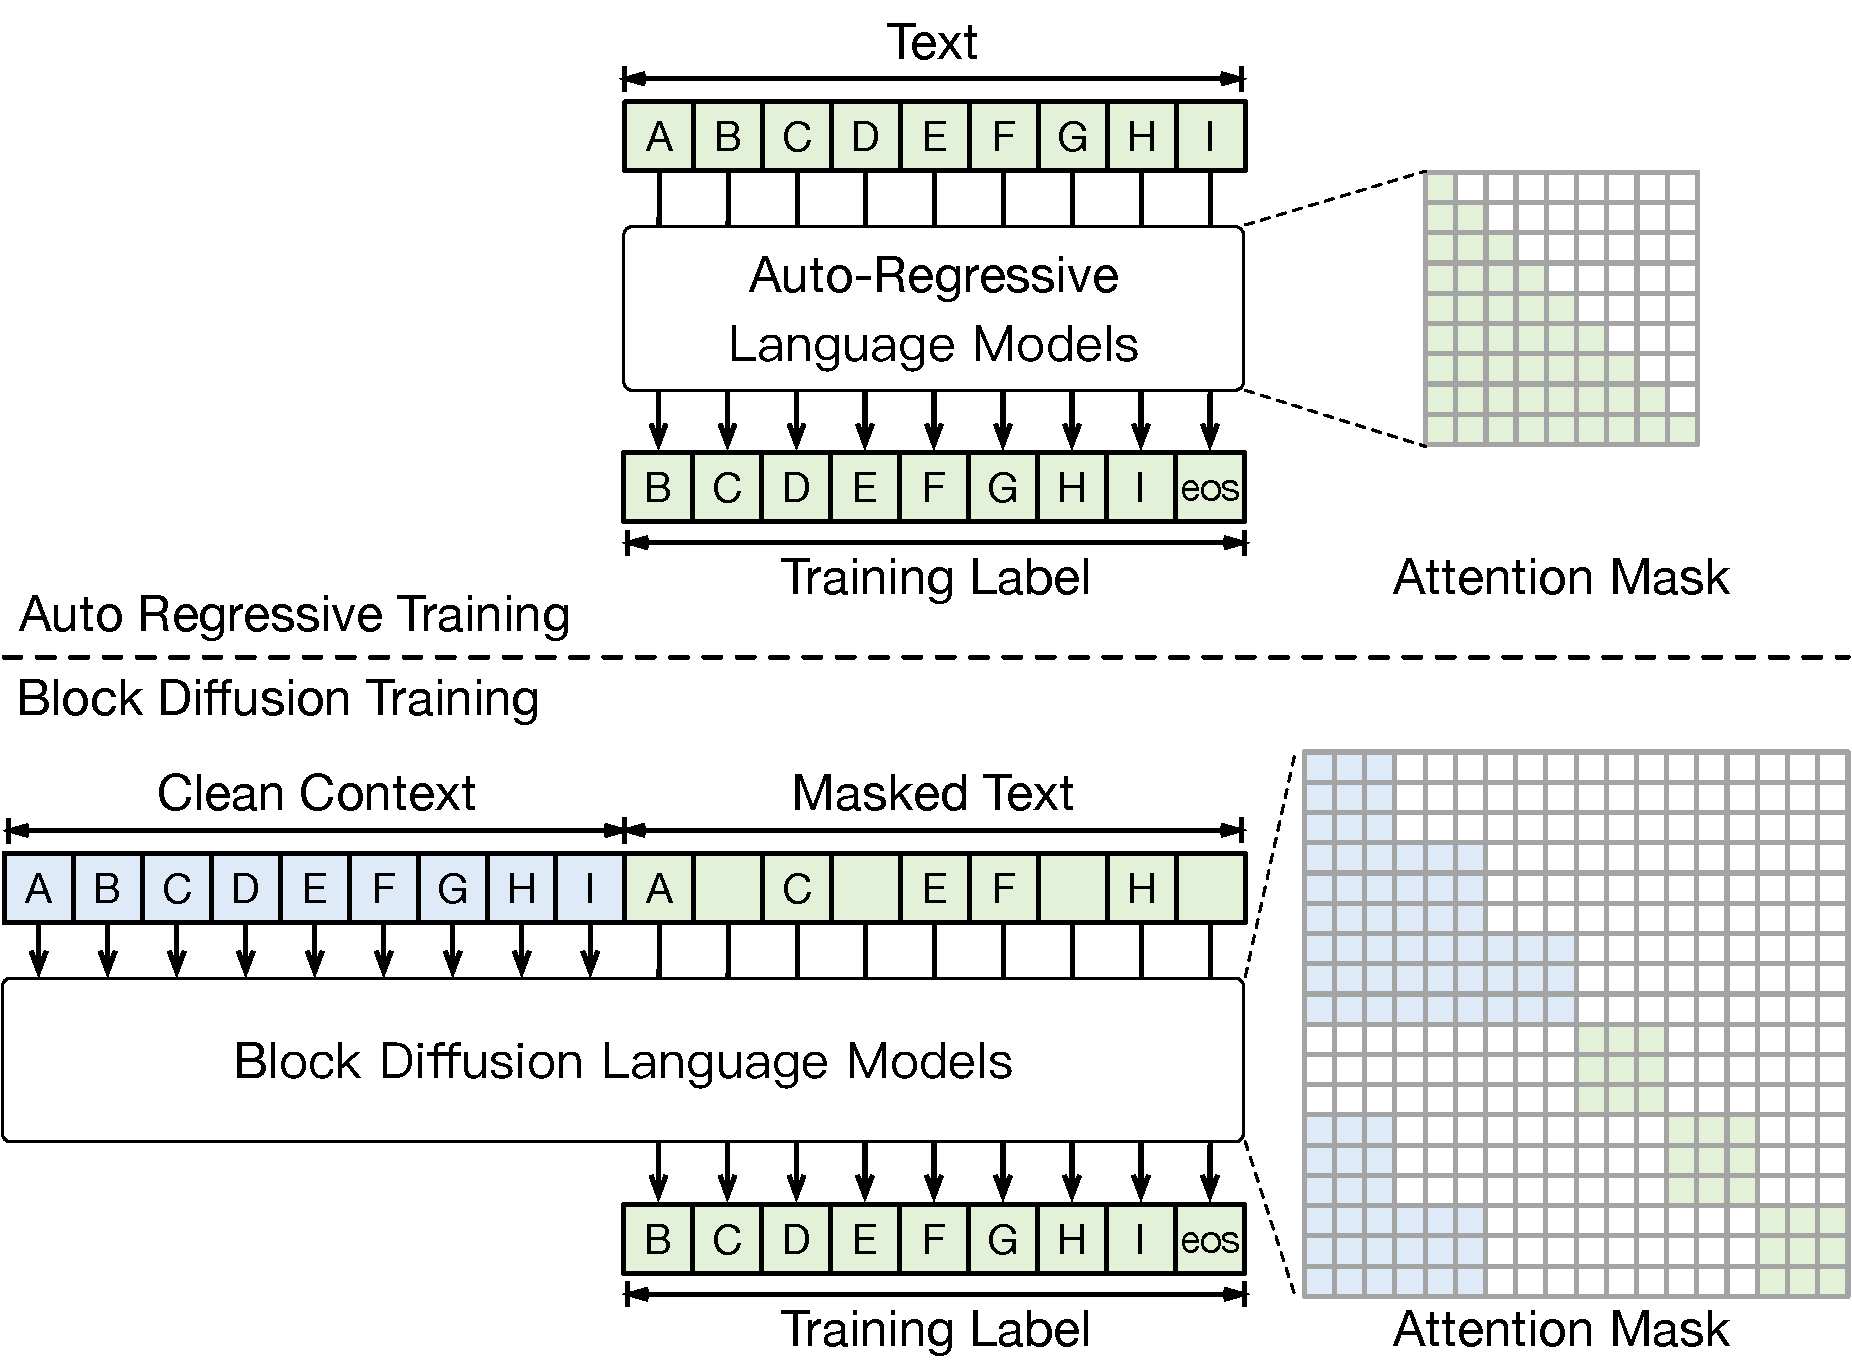
\includegraphics[width=0.47\textwidth]{figures/original_pattern.pdf}
    \caption{The training pattern of Auto-Regressive Language Models and Block Diffusion Language Models.}
    \label{fig:original_pattern}
\end{figure}

\begin{figure*}[t]
    \centering
    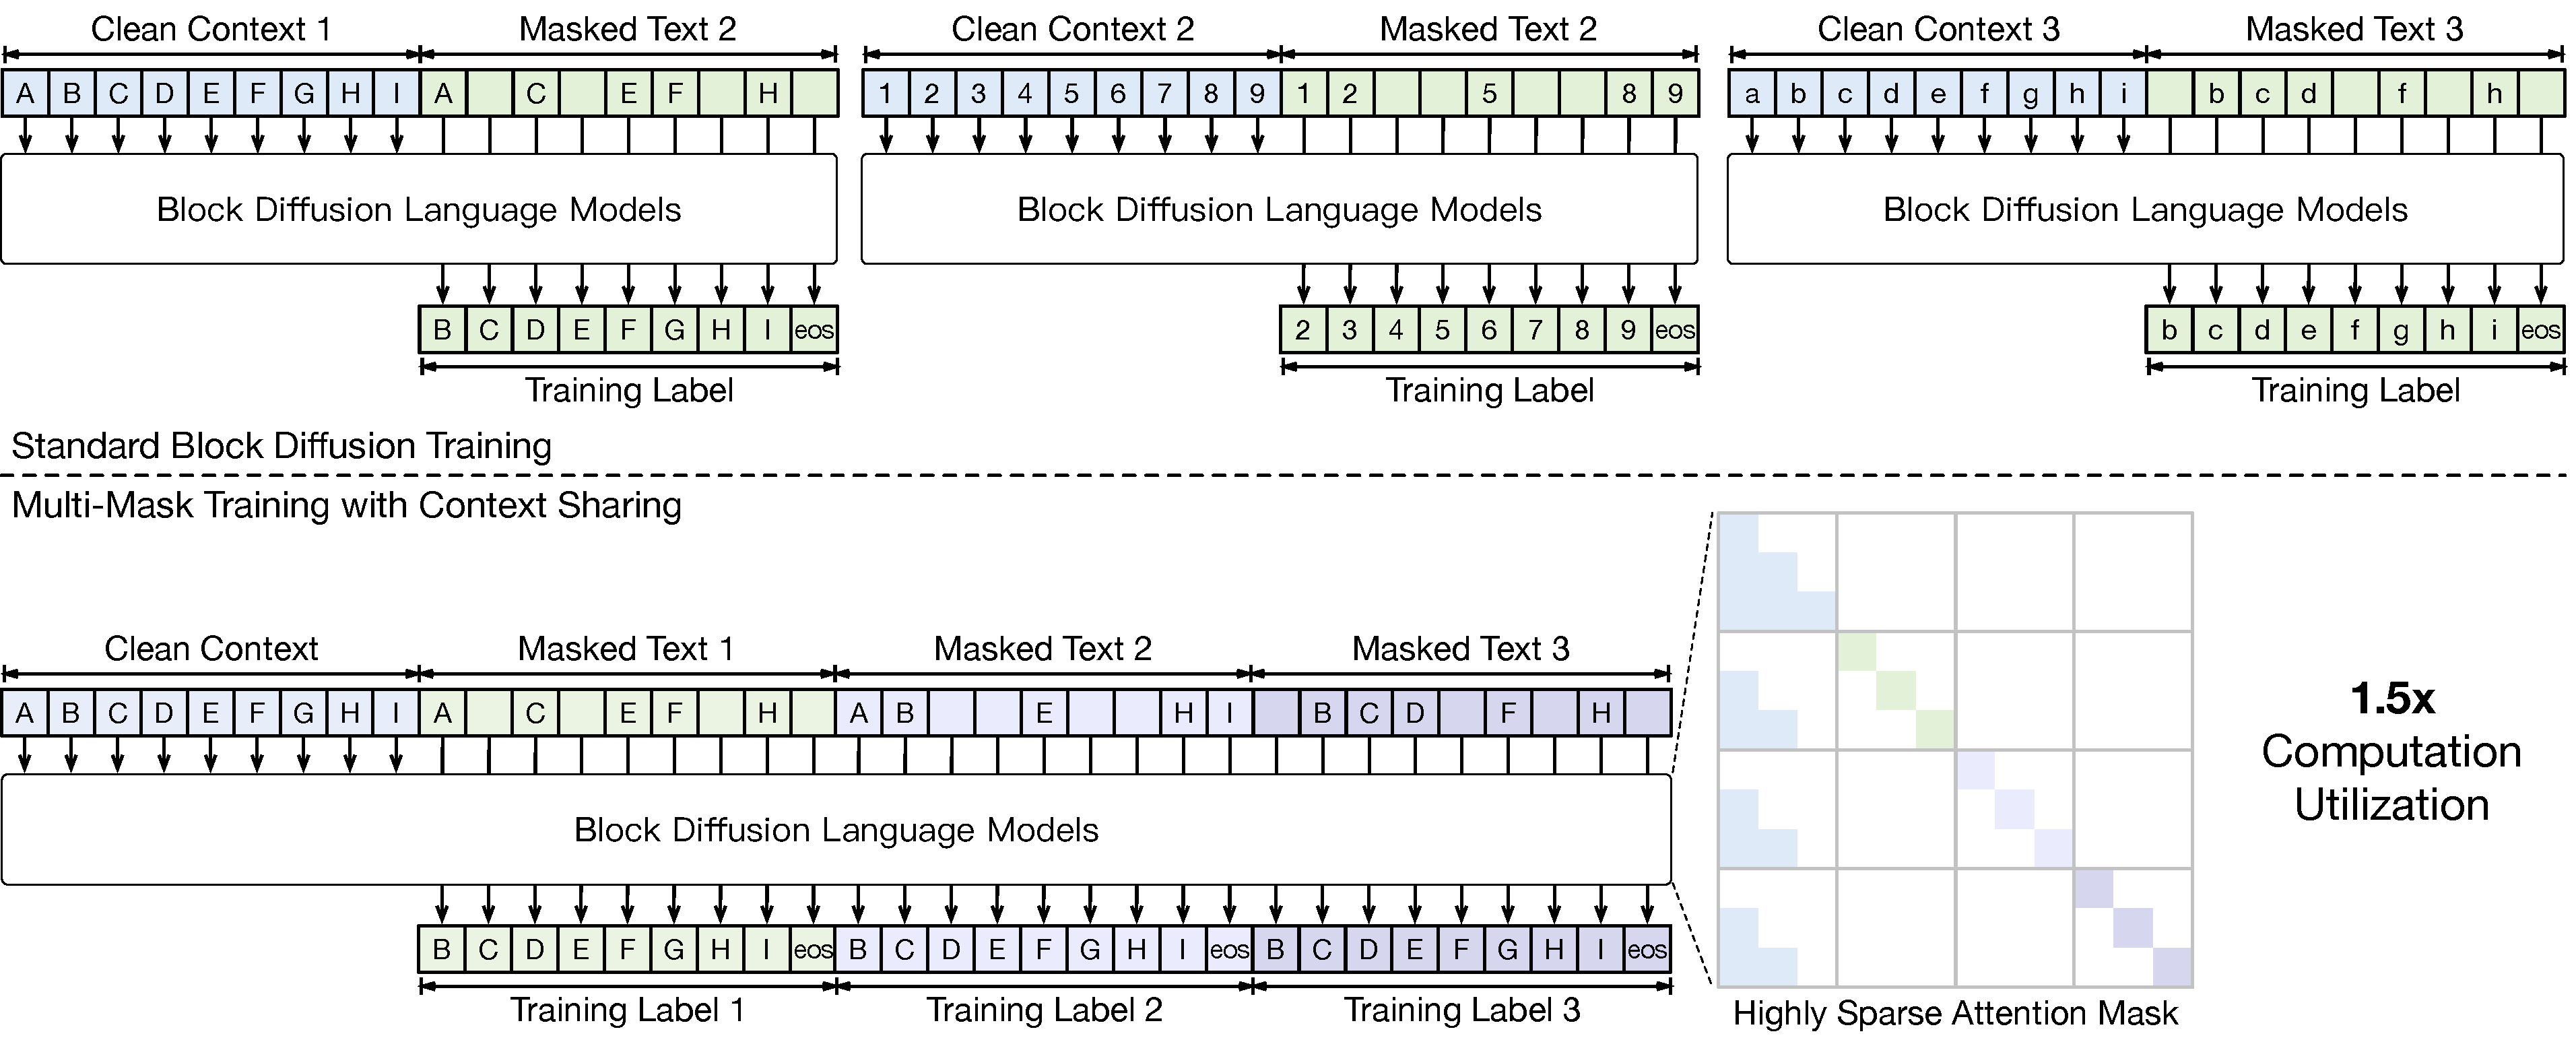
\includegraphics[width=0.95\textwidth]{figures/new_pattern.pdf}
    \caption{The training pattern of \name{} compared to the original training pattern of Block Diffusion Language Models, when the number of different mask patterns $K$ is $3$. MMT train on less training instance but instead train on more mask patterns.}
    \label{fig:method}
\end{figure*}

The success of Large Language Models~\citep{gpt3,foundation-model,PTMs-survey,gpt4} has been largely driven by autoregressive (AR) architectures.
However, their sequential, token-by-token generation paradigm imposes significant latency bottlenecks during inference.
Recently, Diffusion Language Models~\citep{llada,mercury,seeddiffusion,geminidiffusion} have emerged as promising alternatives.
By training the model to generate tokens in parallel, these models offer a flexible trade-off between generation quality and inference speed.

Block Diffusion Language Models~\citep{bd3lms,fastdllmv2,sdar,nbdiff,llada2} further bridge the gap between autoregressive and diffusion paradigms.
These models decompose the generation process into sequential blocks, where tokens within each block are generated via diffusion while blocks themselves are produced autoregressively.
This hybrid formulation enables variable-length generation, supports KV caching across blocks, and allows parallel token sampling within each block, making it a compelling architecture for practical deployment.

Despite their promising inference properties, Block Diffusion Language Models suffer from a critical training inefficiency.
As illustrated in Figure~\ref{fig:original_pattern}, each training sample is duplicated into two copies: one serves as the clean context, while the other is masked and used for loss computation.
This duplication results in a mere 50\% computational utilization, as half of the forward pass is spent on the context that does not contribute to the training signal.
In contrast, autoregressive models achieve near-100\% utilization since every token contributes to the training loss.
Beyond the wasted FLOPs, this inefficiency also incurs substantial memory and I/O overhead: the clean context occupies precious GPU memory during forward and backward passes, yet contributes zero gradients to the model update.

In this paper, we propose \textbf{\NAME{} with context sharing} (\textbf{\name{}}), a simple yet effective training paradigm that significantly improves computational utilization through a carefully designed attention mechanism.
Our key insight is that instead of processing one mask pattern per sample, we can generate $K$ different mask patterns for the same clean text and process them together in a single forward pass.
As illustrated in Figure~\ref{fig:method}, by concatenating the shared clean prefix with $K$ masked suffixes and employing a \emph{context-sharing attention mask}, each masked segment attends to the clean context while remaining isolated from other segments.
The resulting attention mask is highly sparse and can be efficiently implemented with FlexAttention~\citep{flexattention}.
This design amortizes the cost of the clean context across $K$ perturbations, improving the computational utilization from $50\%$ to $\frac{K}{1+K}$.
Crucially, we find that when using appropriate number of mask patterns $K$, \textbf{training on fewer samples with multiple perturbations per sample} yields comparable or even better model quality than training on more samples with single perturbations.
Intuitively, by exposing the model to $K$ different mask patterns of the same underlying text within a single forward pass, \name{} acts as an implicit ensemble over perturbations, reducing the variance of the gradient signal and leading to more stable optimization.
This \emph{variance reduction} effect explains why \name{} can achieve faster training without sacrificing or even improving model quality.

Beyond training, our context-sharing attention mask can also accelerate inference in diffusion-based reinforcement learning (RL).
In diffusion RL, evaluating the probability of generated text requires Monte-Carlo sampling over multiple mask patterns, which is computationally expensive when performed naively.
By batching these mask patterns together and applying our sparse attention mechanism, we can significantly reduce the cost of probability estimation during policy optimization.

Our contributions are summarized as follows:
\begin{itemize}[parsep=0pt,itemsep=3pt,topsep=0pt]
    \item We identify the low computational utilization in Block Diffusion training, where the clean context incurs computation but does not contribute to the loss.
    \item We propose \name{}, a multi-mask training paradigm with context sharing that processes multiple masked perturbations of the same sample in a single forward pass via a specially designed sparse attention pattern.
    \item Experiments show that \name{} accelerates Block Diffusion training by $1.6\times$ with no loss in perplexity (TODO) or downstream task performance.
\end{itemize}
